\documentclass{article}
\usepackage[utf8]{inputenc}
\usepackage[english]{babel}
\usepackage[letterpaper,top=2cm,bottom=2cm,left=3cm,right=3cm,marginparwidth=1.75cm]{geometry}
\usepackage{amsmath}
\usepackage{tikz}
\usepackage{graphicx}
\usepackage{bigints}
\usepackage{amssymb}
\usepackage[colorlinks=true, allcolors=blue]{hyperref}

\DeclareMathOperator{\vol}{vol}
\DeclareMathOperator{\osc}{osc}
\newcommand{\reals}{\mathbb{R}}
\newcommand{\rationals}{\mathbb{Q}}
\newcommand{\integers}{\mathbb{Z}}
\newcommand{\dypaving}{\mathcal{D}_N}


\title{Math 31CH HW1 \\ Due April 5 at 11:59 pm by Gradescope Submission}
\author{Merrick Qiu}


\begin{document}
\maketitle
\newpage



\subsection*{Exercise 4.1.9}
Let $Q 
% \in % \in means "an element of"
\subset 
\mathbb{R}^2$ be the unit square $0 \leq x, y < 1$.\footnote{Note that we slightly changed the exercise from the book's version, which actually makes it simpler.} Show that the function
$$f\begin{pmatrix} x\\y\end{pmatrix}  = \sin(x - y)
% 1_Q
\,
\mathbf{1}_Q
\begin{pmatrix} x\\y\end{pmatrix}$$
is integrable by providing an explicit bound for $U_N(f) - L_N(f)$ that tends to $0$
as $N \to \infty$.\medskip 

\textbf{Solution.}
The inequality $|\sin(x_2)-\sin(x_1)| \leq |x_2 - x_1|$ 
(i.e. Lipschitzs continuous with $C=1$)
provides a bound for the oscilation of any dyadic cube $C_{k, N}$.
For some $(x_2, y_2)$ and $(x_1, y_1)$ in $\overline{C}$,
\begin{align*}
    \osc_C(f)
    &= |\sin(x_2-y_2)-\sin(x_1-y_1)| \\
    &\leq |(x_2-y_2)-(x_1-y_1)| \\
    &= |(x_2-x_1)-(y_2-y_1)| \\
    &\leq |x_2-x_1| + |y_2-y_1| \\
    &= \frac{1}{2^N} + \frac{1}{2^N} \\ 
    &= \frac{1}{2^{N-1}}
\end{align*}

In the dyadic paving $\dypaving$, 
there are $2^{2N}$ dyadic cubes 
with a volume of $\frac{1}{2^{2N}}$.
So $U_N(f) - L_N(f)$ is bounded by $\frac{1}{2^{N-1}}$ since 
\begin{align*}
    U_N(f) - L_N(f)
    &= \sum_{C \in \dypaving} \osc_C(f) \vol_2 C \\
    &\leq \sum_{C \in \dypaving} \frac{1}{2^{N-1}} \frac{1}{2^{2N}} \\
    &= 2^{2N} \frac{1}{2^{N-1}} \frac{1}{2^{2N}} \\
    &= \frac{1}{2^{N-1}}
\end{align*}

Since $\frac{1}{2^{N-1}}$ tends to 0 as $N \to \infty$,
$U_N(f) - L_N(f)$ tends to 0 as $N \to \infty$,
and so $f$ is integrable.
\newpage

\subsection*{Exercise 4.1.10}

\textbf{a.} What are the upper and lower sums $U_1(f)$ and $L_1(f)$ for the function
$$f\begin{pmatrix} x\\y\end{pmatrix} = \begin{cases}
      x^2 + y^2 & \text{if}\ 0<x,y<1 , \\
      0 & \text{otherwise},
    \end{cases}$$
    i.e., the upper and lower sums for the partition $\mathcal{D}_1(\mathbb{R}^2)$, shown in the figure at
left (below actually)? 

\begin{figure}[ht!]
    \centering
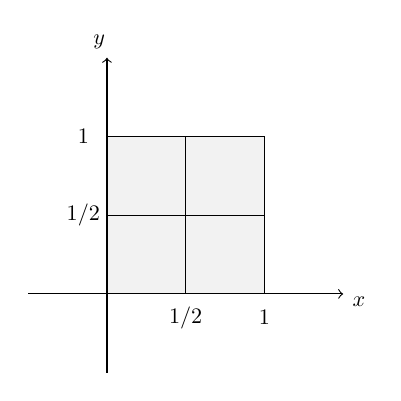
\begin{tikzpicture}
\filldraw[gray!10] (0,0) -- (2,0) -- (2,2) -- (0,2) ;
\draw[->] (-1,0) -- (3,0) ;
\draw[->] (0,-1) -- (0,3) ;
\draw (2,0) -- (2,2) -- (0,2) ;
\draw (1,0) -- (1,2) ;
\draw (0,1) -- (2,1) ;
\node[scale=.8] at (1,-.3) {$1/2$} ;
\node[scale=.8] at (2,-.3) {$1$} ;
\node[scale=.8] at (-.3,1) {$1/2$} ;
\node[scale=.8] at (-.3,2) {$1$} ;
\node[scale=.8] at (3.2,-.1) {$x$} ;
\node[scale=.8] at (-.1,3.2) {$y$} ;
\end{tikzpicture}
    \caption{Figure for Exercise 4.1.10.}
    \label{fig:my_label 1}
\end{figure}


\medskip 

\textbf{Solution to (a).}
Since $f$ monotonically increases as $x$ increases or $y$ increases,
the supremum of the dyadic cube occurs at the top right of the cube, and
the infinum of the dyadic cubes occurs at the bottom left of the cube.

\[
    U_1(f) 
    = \frac{1}{4}(\frac{1}{2} + \frac{5}{4} + \frac{5}{4} + 2)
    = \frac{5}{4}
\]
\[
    L_1(f) 
    = \frac{1}{4}(0 + \frac{1}{4} + \frac{1}{4} + \frac{1}{2})
    = \frac{1}{4}
\]

\bigskip 

% \subsection{Problem b}
\textbf{b.}  Compute the integral of $f$ and show that it is between the upper and lower sums.
\medskip 

\textbf{Solution to (b).}
Using Fubini's theorem, the integral can be written as 
\[
    \int_{\reals^2} f |dxdy|
    =\int_{-\infty}^\infty (\int_{-\infty}^\infty f(x, y) \,dx) \,dy
    = \int_0^1 (\int_0^1 x^2+y^2 \,dx) \,dy
\]

This can then be solved using single-variable calculus
\begin{align*}
    \int_0^1 (\int_0^1 x^2+y^2 \,dx) \,dy
    &= \int_0^1 \left[\frac{x^3}{3} + xy^2\right]_{x=0}^{x=1} \,dy \\
    &= \int_0^1 \frac{1}{3} + y^2 \,dy \\
    &= \left[ \frac{y}{3} + \frac{y^3}{3} \right]_{y=0}^{y=1} \\
    &= \frac{2}{3}
\end{align*}
The integral is between the upper and lower sums since
\[
    \frac{1}{4} \leq \frac{2}{3} \leq \frac{5}{4}
\]
\newpage

\subsection*{Exercise 4.1.14, Part a.}

Consider the function
$$f(x) = \begin{cases}
      \; 0 & \text{if}\ x\notin [0,1] \text{, or }x \text{ is rational}, \\
      \; 1 & \text{if}\ x\in [0,1] \text{, and }x \text{ is irrational}.
    \end{cases}$$
What value do you get for the ``left Riemann sum'', where for the interval
$ C_{k,N} = \Big\{ x \Big| \frac{k}{2^N} < x <\frac{k+1}{2^N}\Big\}$
you choose the left endpomt $\frac{k}{2^N}$?  For the sum you get when you choose the right endpoint $\frac{k+1}{2^N}$? The midpoint Riemann sum?
\medskip 

\textbf{Solution.}
\begin{enumerate}
    \item 
    The inverval $C_{k_N}$ will have a left Riemann sum of 0 
    since $k \in \integers$ implies the rationality of the left endpoint, 
    $\frac{k}{2^N} \in \rationals$. 
    \item 
    The inverval $C_{k_N}$ will have a right Riemann sum of 0 
    since $k \in \integers$ implies the rationality of the right endpoint, 
    $\frac{k+1}{2^N} \in \rationals$. 
    \item 
    The inverval $C_{k_N}$ will have a midpoint Riemann sum of 0
    since $k \in \integers$ implies the rationality of the midpoint, 
    $\frac{k+\frac{1}{2}}{2^N} \in \rationals$.
\end{enumerate}



\newpage

\subsection*{Exercise 4.5.6}
\textbf{Part a.}
Show that as $n$ increases, the volume of the $n$-dimensional unit \emph{ball} becomes a smaller and smaller proportion of the smallest $n$-dimensional cube that contains it.\footnote{The book uses the word ``sphere'' instead of ``ball''.}
\medskip 

\textbf{Solution.}
The volume of the n-dimensional cube that contains the unit sphere is $2^n$.
Let $\beta_n$ be the volumen of the n-dimensional unit sphere.
Let $c_n$ be defined such that $\beta_{n} = c_n\beta_{n-1}$.
In order to show that the proportion of the sphere decreases,
it is sufficient to show that $c_n < 2$ for all $n>1$ since
\[
    \frac{\beta_n}{2^n} < \frac{\beta_{n-1}}{2^{n-1}}
    \iff \frac{c_n\beta_{n-1}}{2^n} < \frac{\beta_{n-1}}{2^{n-1}}
    \iff c_n < 2
\]

From exercise 4.5.4, 
\[
    c_n = \frac{n-1}{n} c_{n-2}
\]
Since $c_0 = \pi$, $c_1 = 2$, and $\frac{n-1}{n} < 1$ for $n>0$,
$c_n < 2$ must be true for all $n>1$.
Therefore, the volume of a n-sphere decreases 
in proportion to the cube that contains it.
\bigskip 

\noindent \textbf{Part b.}
What is the first $n$ for which the ratio of volumes is smaller than $10^{-2}$?
\medskip 

\textbf{Solution.}
From exercise 4.5.5,
the volume of a unit sphere in n-dimensions 
if n is even is 
\[
    \beta_n = \beta_{2k}
    = \frac{\pi^k}{k!} 
\] 
If n is odd, the volume is 
\[
    \beta_n = \beta_{2k+1}
    = \frac{\pi^k k! 2^{2k+1}}{(2k+1)!} 
\] 
The inequality $\frac{\pi^k}{2^{2k} k!} < 10^{-2}$ is first true at $k=5$
which corresponds to $n=10$. \\
The inequality $\frac{\pi^k k!}{(2k+1)!} < 10^{-2}$ is first true at $k=4$
which corresponds to $n=9$. \\
Therefore, $n=9$ is the first $n$ for which the ratio is smaller than $10^{-2}$.
\bigskip 

\noindent \textbf{Part c.}
What is the first $n$ for which it is smaller than $10^{-6}$?
\medskip 

\textbf{Solution.}

The inequality $\frac{\pi^k}{2^{2k} k!} < 10^{-6}$ is first true at $k=9$
which corresponds to $n=18$. \\
The inequality $\frac{\pi^k k!}{(2k+1)!} < 10^{-6}$ is first true at $k=9$
which corresponds to $n=19$. \\
Therefore, $n=18$ is the first $n$ for which the ratio is smaller than $10^{-6}$.
\newpage

\subsection*{Exercise 4.5.7}
Write as an iterated integral, and in six different ways, the triple integral of $xyz$ over the region $x, y, z \geq 0,\; x + 2y + 3z \leq 1$. You need not compute the integrals.
\medskip 

\textbf{Solution.}
\begin{enumerate}
    \item
    \[
        \int_{0}^{1} \int_{0}^{\frac{1}{2}(1-x)} \int_{0}^{\frac{1}{3}(1-x-2y)}  \,dz \,dy \,dx
    \]
    \item
    \[
        \int_{0}^{\frac{1}{2}} \int_{0}^{(1-2y)} \int_{0}^{\frac{1}{3}(1-x-2y)}  \,dz \,dx \,dy
    \]
    \item
    \[
        \int_{0}^{1} \int_{0}^{\frac{1}{3}(1-x)} \int_{0}^{\frac{1}{2}(1-x-3z)}  \,dy \,dz \,dx
    \]
    \item
    \[
        \int_{0}^{\frac{1}{3}} \int_{0}^{1-3z} \int_{0}^{\frac{1}{2}(1-x-3z)}  \,dy \,dx \,dz
    \]
    \item
    \[
        \int_{0}^{\frac{1}{2}} \int_{0}^{\frac{1}{3}(1-2y)} \int_{0}^{1-2y-3z}  \,dx \,dz \,dy
    \]
    \item
    \[
        \int_{0}^{\frac{1}{3}} \int_{0}^{\frac{1}{2}(1-3z)} \int_{0}^{1-2y-3z}  \,dx \,dy \,dz
    \]
\end{enumerate}
\newpage

\subsection*{Exercise 4.5.12}
\textbf{Part a.}
Represent the iterated integral $\displaystyle \int_0^a \left(\int_{x^2}^{a^2}\sqrt{y}\,e^{-y^2}dy\right) dx$ as the integral of $\sqrt{y}\,e^{-y^2}$ over a region of the plane. Sketch this region.
\medskip 

\textbf{Solution.}
\begin{figure}[ht!]
    \centering
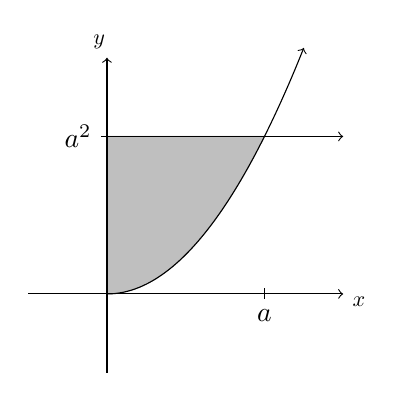
\begin{tikzpicture}
\filldraw[gray!50] plot[smooth,domain=0:2] (\x, {\x*\x/2}) -| (0, 2);
\draw[->] (-1,0) -- (3,0) ;
\draw[->] (0,-1) -- (0,3) ;
\draw[->] (0,2) -- (3,2) ;
\draw[->] plot[smooth,domain=0:2.5] (\x, {\x*\x/2});
\draw (2,2pt)--(2,-2pt) node[below] {$a$};
\draw (2pt,2)--(-2pt,2) node[left] {$a^2$};
\node[scale=.8] at (3.2,-.1) {$x$} ;
\node[scale=.8] at (-.1,3.2) {$y$} ;
\end{tikzpicture}
    \caption{Figure for Exercise 4.5.12.a}
    \label{fig:my_label 2}
\end{figure}
\bigskip

\textbf{Part b.}
Use Fubini's theorem to make this integral into an iterated integral in the opposite order.
\medskip 

\textbf{Solution.}
\[
    \int_{0}^{a^2} \int_{0}^{\sqrt{y}} \sqrt{y} e^{-y^2} \,dx \,dy
\]
\bigskip

\textbf{Part c.}
Evaluate the integral.
\medskip 

\textbf{Solution.}
\begin{align*}
    \int_{0}^{a^2} \int_{0}^{\sqrt{y}} \sqrt{y} e^{-y^2} \,dx \,dy
    &= \int_{0}^{a^2} \left[ \sqrt{y} e^{-y^2}x \right]_{x=0}^{x=\sqrt{y}} \,dy \\
    &= \int_{0}^{a^2} y e^{-y^2}  \,dy \\ 
    &= \left[ -\frac{1}{2}e^{-y^2} \right]_{y=0}^{y=a^2} \\
    &= \frac{1}{2}-\frac{1}{2}e^{-a^4}
\end{align*}
\newpage

\subsection*{Exercise 4.5.15}
Find the volume of the region
$$z \geq x^2 + y^2 , \quad  z \leq 10 - x^2 - y^2 . $$
\medskip 

\textbf{Solution.}


In cylindrical coordinates, 
$z=x^2+y^2 = \sqrt{x^2+y^2}^2 = r^2$.
The volume can be found by multiplying half of the volume by 2.
The integral can be written as
\[
    2\int_{0}^{2\pi} 
    \int_{0}^{\sqrt{5}} 
    \int_{0}^{r^2} 
    r \,dz \,dr \,d\theta
\]

\begin{align*}
    2\int_{0}^{2\pi} \int_{0}^{\sqrt{5}} 
        \int_{0}^{r^2} r \,dz \,dr \,d\theta 
    &= 2\int_{0}^{2\pi} \int_{0}^{\sqrt{5}} 
        \left[ rz \right]_{z=0}^{z=r^2} \,dr \,d\theta \\
    &= 2\int_{0}^{2\pi} \int_{0}^{\sqrt{5}} r^3 \,dr \,d\theta \\
    &= 2\int_{0}^{2\pi} 
        \left[\frac{r^4}{4}\right]_{r=0}^{r={\sqrt{5}}} \,d\theta \\
    &= 2\int_{0}^{2\pi} \frac{25}{4}\,d\theta \\
    &= 2\frac{25\pi}{2} \\
    &= 25\pi
\end{align*}
%\newpage
% \subsection*{Proof for volume of unit n-sphere for exercise 4.5.6}
% \textbf{Solution.}
% Let $B^n_R(0)$ be a sphere of radius $R$ centered at $0$ in $\reals^n$, and
% let $b_n(R)$ be the volume of the sphere.
% Let $\beta_n = b_n(1)$ be the volume of the unit sphere in n dimensions.
% Integrating over the slices of the sphere and using $b_n(R) = R^nb_n(1)$, 
% \begin{align*}
%     \beta_n
%     &= \int_{B_1^n(0)} |d^nx| \\ 
%     &= \int_{-1}^1 (\int_{B_{\sqrt{1-x_n^2}}^{n-1}(0)} |d^{n-1}x|) \,dx_n \\
%     &= \int_{-1}^1 b_{n-1} (\sqrt{1-x_n^2}) \,dx_n \\ 
%     &= \int_{-1}^1 (\sqrt{1-x_n^2})^{n-1} b_{n-1}(1) \,dx_n \\ 
%     &= \beta_{n-1} \int_{-1}^1 (1-x_n^2)^{\frac{n-1}{2}}  \,dx_n \\ 
% \end{align*}

% Let $c_n = \int_{-1}^1 (1-t^2)^{\frac{n-1}{2}}  \,dt$,
% so the above relation can be written as $\beta_n = c_n \beta_{n-1}$.
% Induction can be used to find the value of $c_n$.
% The base cases are $c_0 = \pi$ and $c_1 = 2$ since 
% \[
%     c_0 
%     = \int_{-1}^1 (1-t^2)^{-\frac{1}{2}}  \,dt
%     = \left[ \sin^{-1}(t) \right]_{t=-1}^{t=1}
%     = \pi
% \]
% \[
%     c_1 
%     = \int_{-1}^1 (1-t^2)^0  \,dt
%     = \int_{-1}^1 \,dt
%     = 2
% \]

% For $n \geq 2$, using integration by parts shows
% \begin{align*}
%     c_n 
%     &= \int_{-1}^1 (1-t^2)^{\frac{n-1}{2}}  \,dt \\
%     &= \left[ t(1-t^2)^{\frac{n-1}{2}} \right]_{t=-1}^{t=1}+
%         (n-1) \int_{-1}^1 t^2(1-t^2)^{\frac{n-3}{2}} \,dt \\ 
%     &= (n-1) \int_{-1}^1 (1-(1-t^2))(1-t^2)^{\frac{n-3}{2}} \\
%     &= (n-1) \int_{-1}^1 (1-t^2)^{\frac{n-3}{2}} - 
%         (n-1) \int_{-1}^1 (1-t^2)^{\frac{n-1}{2}} \\
%     &= (n-1)c_{n-2}-(n-1)c_n
% \end{align*}

% Therefore for $n \geq 2$,
% \[
%     c_n = \frac{n-1}{n} c_{n-2}
% \]
% From this, the values of $c_n$ can be found for even indexes with 
% \[
%     c_{2k} = c_0 \prod_{i=1}^k \frac{2i-1}{2i}
% \]
% and for odd indexes 
% \[
%     c_{2k+1} = c_1 \prod_{i=1}^k \frac{2i}{2i+1}
% \]

% Using $\beta_n = c_n \beta{n-1}$, 
% the values of $\beta_n$ can be found inductively for the even indexes.
% Assume that  $\beta_{2k} = \frac{\pi^k}{k!}$.
% From this,
% \begin{align*}
%     \beta_{2k+2} 
%     &= c_{2k+2}c_{2k+1}\beta_{2k} \\
%     &= c_0 \prod_{i=1}^{k+1} (\frac{2i-1}{2i}) 
%        c_1 \prod_{i=1}^k (\frac{2i}{2i+1})
%         \frac{\pi^k}{k!} \\
%     &=  \frac{2k+1}{2k+2} c_0 c_1
%         \prod_{i=1}^{k} \frac{2i-1}{2i+1}
%         \frac{\pi^k}{k!} \\ 
%     &=  \frac{2k+1}{2k+2} c_0 c_1
%         \frac{1}{2k+1}
%         \frac{\pi^k}{k!} \\ 
%     &= \frac{\pi}{k+1} \frac{\pi^k}{k!} \\ 
%     &= \frac{\pi^{k+1}}{(k+1)!} \\
% \end{align*}

% Since $\beta_2 = \pi$ for the base case,
% $\beta_{2k} = \frac{\pi^k}{k!}$ for all $k>0$.

% The value of $\beta_{2k+1}$ can be found by finding $c_{2k+1}$
% The following products can be written as
% \[
%     \prod_{i=1}^k 2i = 2^k k!
% \]
% \[
%     \prod_{i=1}^k 2i+1 
%     = \frac{(2k+1)!}{\prod_{i=1}^k 2i}
%     = \frac{(2k+1)!}{2^k k!}
% \]

% Therefore,
% \[
%     c_{2k+1} 
%     = c_0\prod_{i=1}^k \frac{2i}{2i+1} 
%     = 2\frac{2^k k!}{\frac{(2k+1)!}{2^k k!}}
%     = \frac{2^{2k+1} k!^2}{(2k+1)!}
% \]

% This gives
% \begin{align*}
%     \beta_{2k+1}
%     &= c_{2k+1}\beta{2k} \\
%     &= \frac{2^{2k+1} k!^2}{(2k+1)!} \frac{\pi^k}{k!} \\
%     &= \frac{\pi^k k! 2^{2k+1}}{(2k+1)!}
% \end{align*}

% Therefore, $\beta_{2k+1} = \frac{\pi^k k! 2^{2k+1}}{(2k+1)!}$ for $k>0$
% (the case $k=1$ can be manually checked).
\end{document} 
